\begin{Large} 
	\textbf{Задача 1}\\
	
	 \end{Large} 
Задача заключалась в реализации следующих функий в классе: (был выбран ЯП Python, полный листинг кода см. в приложении А)
\begin{itemize}
	\item Ввод матрицы заданного размера пользователем.
	\item Подсчет следа матрицы.
	\item Поиск и вывод элемента матрицы по заданным индексам.
	\item Тестирование работы программы и создание консольного пользовательского интерфейса.\\
\end{itemize}

\begin{large}
	Использованные библиотеки и инструменты языка\\
\end{large}
В ходе написания программы были использованы только стандартные средства языка. Также для удобства и лучшей читаемости кода была импортирована библиотека typing.\\

\begin{large}
	Реализация функций и основные идеи\\
\end{large}
Все функции были реализованы в классе MatrixKeeper\\\\
Написаны функции:\\
inputMatrix - ввод матрицы пользователем,\\
trace - поиск следа матрицы,\\
findByIndex - поиск элемента по введенному индексу.\\

Суть работы алгоритмов:
\begin{itemize}
	\item inputMatrix: Приглашение пользователя ко вводу. Вначале через пробел вводятся два числа типа int - размер матрицы. Вторым приглашением вводится матрица по строке, элементы в строке разделяются пробелом.
	\item trace: След матрицы - сумма элементов главной диагонали этой матрицы. Циклом, оставаясь в пределах матрицы, проходимся по элементам с индексами вида [i][i], считаем сумму таких элементов. Можем так делать по той причине, что матрица имеет следующую структуру в классе:\vspace{3cm}
	\begin{lstlisting} [language=Python]
		self.matrix: Optional[List[List[float]]]
		\end{lstlisting} - то есть храним матрицу как список, каждый элемент которого является тоже списком.
	\item findByIndex: возвращаем элемент из матрицы, отнимая от индексов по единице, т.к. в ЯП отсчет начинается с нуля.
	\begin{lstlisting}
		return self.matrix[n-1][m-1]
	\end{lstlisting}
\end{itemize}
\begin{large}
	Тестирование программы\\
\end{large}
Написаны юниттесты для каждой функции класса с помощью стандартной библиотеки unittest. Также протестировано вручную.\\
Листинг кода теста см. в приложении А-test.\\
\begin{figure}[H]
	\centering
	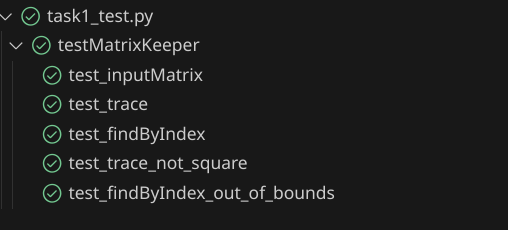
\includegraphics[width=0.5\linewidth]{tests-task1}
	\caption*{Успешное прохождение unittests}
	\label{fig:tests-task1}
\end{figure}
\begin{figure}[H]
	\centering
	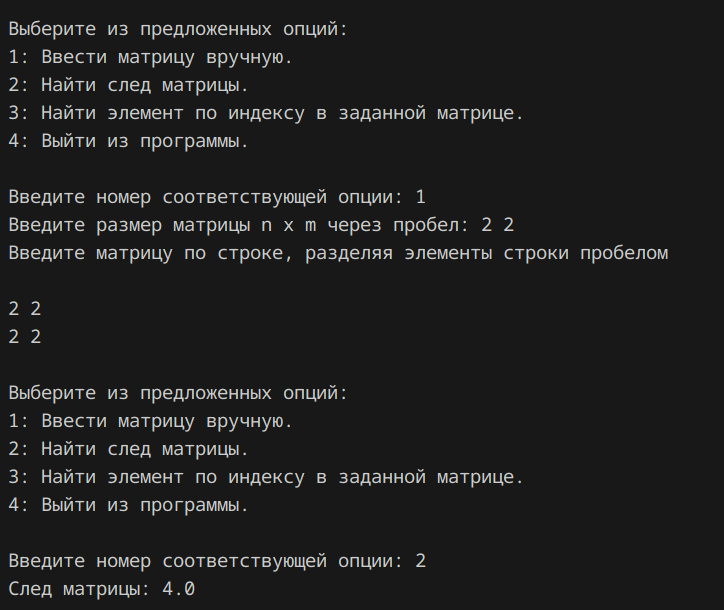
\includegraphics[width=0.5\linewidth]{tests-task2}
	\caption*{Ручной тест поиска следа матрицы 2х2 со всеми элементами, равными 2.}
	\label{fig:tests-task2}
\end{figure}
\begin{figure}[H]
	\centering
	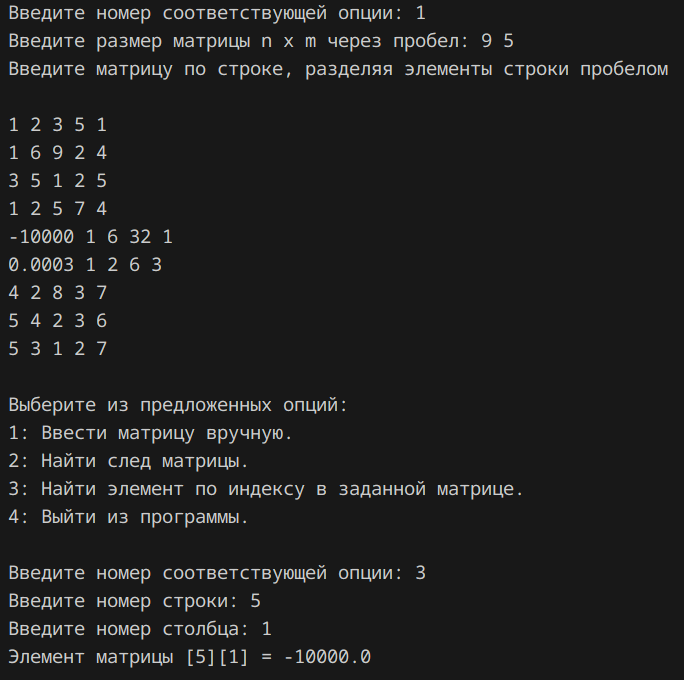
\includegraphics[width=0.5\linewidth]{tests-task3}
	\caption*{Ручной тест поиска страшного элемента в страшной матрице 9х5.}
	\label{fig:tests-task3}
\end{figure}
Итак, справились с первым заданием.\\

\begin{large}
	Задача 2
\end{large}




